\section{Regras}

hasPermission(RHO,GOAL) :- \\ hasObligation(RHO,GOAL).

conditionViol(AGENT,GOAL,CONDITION):- \\ requiresCirc(GOAL,CONDITION),notIsPresent(CONDITION), \\ instanceOfCond(CONDITION),starts(AGENT,GOAL).

relationViol(AGENT,GOAL,RELATION):- \\ requiresCirc(GOAL,RELATION), \\ notIsPresent(RELATION), \\  instanceOfRel(RELATION), \\starts(AGENT,GOAL).

entityViol(AGENT,GOAL,ENTITY) :- \\requiresEntity(GOAL,ENTITY),notIsPresent(ENTITY), \\ starts(AGENT,GOAL).

negConseqFor(GOAL,AGENT,RISK,CONSEQUENCE) :- \\ conditionViol(AGENT,GOAL,CONDITION), \\ hasRisk(CONDITION,RISK,CONSEQUENCE).

negConseqFor(GOAL,AGENT,RISK,CONSEQUENCE) :- \\ relationViol(AGENT,GOAL,RELATION), \\hasRisk(RELATION,RISK,CONSEQUENCE).

possOfNegConseqFor(OTHERRELATION) :- \\ relationViol(AGENT,GOAL,RISK), \\ affectsRels(RELATION,OTHERRELATION).

negConseqFor(GOAL,AGENT,RISK,CONSEQUENCE) :- \\ possOfNegConseqFor(OTHERRELATION), \\ happensNegConseqFor(OTHERRELATION), \\ requiresCirc(GOAL,OTHERRELATION), \\ notIsPresent(OTHERRELATION), \\ isInstanceOfRel(OTHERRELATION), \\ hasRisk(OTHERRELATION,RISK,CONSEQUENCE), \\ starts(AGENT,GOAL).

stopped(GOAL):- \\ entityViol(AGENT,GOAL,ENTITY).

stopped(GOAL) :- \\ negConseqFor(GOAL,AGENT,RISK,CONSEQUENCE).

enabledToStart(AGENT,GOAL) :- \\ adoptsRole(AGENT,RHO), \\ hasPermission(RHO, GOAL), \\ nextGoal(GOAL,NEXTGOAL), \\ reached(GOAL).

stopped(GOAL) :- \\ adoptsRole(AGENT,RHO), \\ hasPermission(RHO, GOAL),\\ lastGoal(GOAL,NEXTGOAL), \\reached(GOAL).


\section{Raciocínio 1}

adoptsRole(agente4,executor2).

hasObligation(executor2,g1).

requiresCirc(g1,relPanoGlicerina).

instanceOfRel(relPanoGlicerina). 

starts(agente4,g1).

notIsPresent(relPanoGlicerina).

affectsRels(relPanoGlicerina,relBastaoGarraCondutor).

affectsRels(relPanoGlicerina,relCordaEstropo).

affectsRels(relPanoGlicerina,relChaveCatracaParafuso).

affectsRels(relPanoGlicerina,relParafusoConector).

affectsRels(relPanoGlicerina,relSoqueteParafuso).

affectsRels(relPanoGlicerina,relAgente4Corda).

affectsRels(relPanoGlicerina,relEstropoCorda).


\section{Raciocínio 2}

adoptsRole(agente2,executor1). 

adoptsRole(agente3,executor1).	 	

adoptsRole(agente4,executor2).	 

hasObligation(executor1,g1).

hasObligation(executor2,g1).

starts(agente2,g1). 

starts(agente3,g1).	 	

starts(agente4,g1).

requiresEntity(g1,pano).		

notIsPresent(pano).

\section{Raciocínio 3}


adoptsRole(agente5,executor3).

hasObligation(executor3,g11).	

starts(agente5,g11).

requiresCirc(g11,umidade70).

instanceOfCond(umidade70).

notIsPresent(umidade70).

hasRisk(umidade70,eletrocutado,morte).

\section{Raciocínio 4}

adoptsRole(agente4,executor2).

hasObligation(executor4,g15).	

starts(agente4,g15).

requiresCirc(g15,relChaveCatracaParafuso).

instanceOfRel(relChaveCatracaParafuso).	

notIsPresent(relChaveCatracaParafuso).

hasRisk(relChaveCatracaParafuso,eletrocutado,morte).

\section{Raciocínio 5}

requiresCirc(g19,relParafusoConector).

hasObligation(executor3,g19).

hasObligation(executor4,g19).

hasObligation(executor5,g19).

starts(agente5,g19).

starts(agente6,g19).

starts(agente7,g19).

adoptsRole(agente5,executor3).

adoptsRole(agente6,executor4).

adoptsRole(agente7,executor5).

hasRisk(relParafusoConector,eletrocutado).

possOfNegConseqFor(relParafusoConector).

happensNegConseqFor(relParafusoConector).

instanceOfRel(relParafusoConector).

hasRisk(relParafusoConector,eletrocutado,morte).

\section{Raciocínio 6}


\begin{figure}[H]
  \centering
  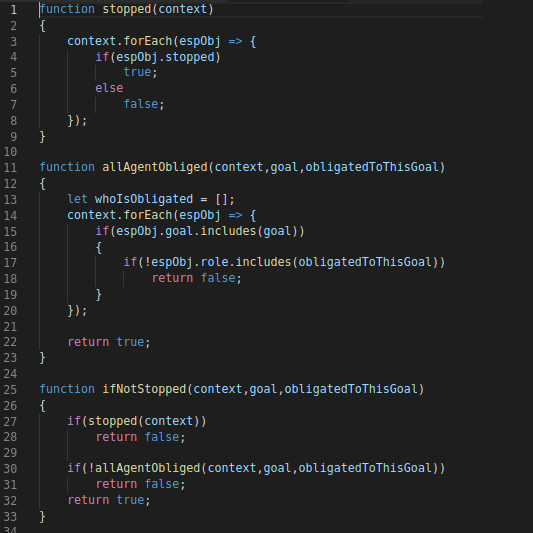
\includegraphics[width=0.8\linewidth]{figure/algjs} 
  \caption{Raciocínio 6 parte 1}
  \label{atividiagram2}
\end{figure}


\begin{figure}[H]
  \centering
  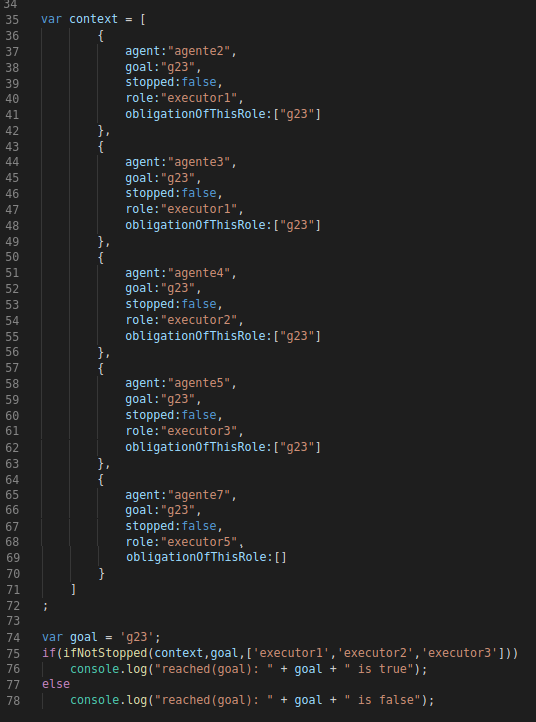
\includegraphics[width=0.8\linewidth]{figure/algjs2} 
  \caption{Raciocínio 6 parte 2}
  \label{atividiagram2}
\end{figure}